\documentclass[12pt,a4paper]{article}

\usepackage[T1]{fontenc}
\usepackage[utf8]{inputenc}
\usepackage[english]{babel}
\usepackage{amsmath}
% Fonts: Libertinus for text and maths, Inconsolata for code
\usepackage[tabular,lining]{libertinus-type1}
\usepackage{libertinust1math}
\usepackage[varqu,varl,scaled=0.95]{zi4}
\usepackage{microtype}
\usepackage[margin=2.5cm, headheight=15pt, headsep=18pt, footskip=28pt]{geometry}
\usepackage{xcolor}
\definecolor{accent}{RGB}{28,63,110}
\definecolor{second}{RGB}{176,58,46}
\definecolor{third}{RGB}{46,125,50}
\definecolor{fourth}{RGB}{214,137,16}
\usepackage{booktabs}
\usepackage[skip=6pt, font=small, labelfont={sf,bf,color=accent}]{caption}
\usepackage{float}
\usepackage{array}
\usepackage{enumitem}
\usepackage{pgfplots}
\pgfplotsset{compat=1.17}
\usepackage{titlesec}
\usepackage{fancyhdr}
\usepackage[colorlinks=true, allcolors=accent,
  pdftitle={SBAM and stochastic matching in dynamic microsimulation}]{hyperref}

\setlist{itemsep=2pt, topsep=4pt}
\setlength{\parindent}{0pt}
\setlength{\parskip}{6pt}
\setlength{\emergencystretch}{2em}
\renewcommand{\arraystretch}{1.15}

\newcommand{\kode}[1]{\texttt{#1}}

% Let tables and figures stay close to the text that refers to them
\renewcommand{\topfraction}{0.9}
\renewcommand{\bottomfraction}{0.7}
\renewcommand{\textfraction}{0.08}
\renewcommand{\floatpagefraction}{0.8}
\setcounter{topnumber}{3}
\setcounter{bottomnumber}{2}
\setcounter{totalnumber}{4}

% Headings
\titleformat{\section}{\sffamily\bfseries\Large\color{accent}}{\thesection}{0.7em}{}
\titleformat{\subsection}{\sffamily\bfseries\large\color{accent}}{\thesubsection}{0.7em}{}
\titlespacing*{\section}{0pt}{20pt plus 4pt minus 2pt}{6pt plus 1pt}
\titlespacing*{\subsection}{0pt}{14pt plus 3pt minus 2pt}{3pt plus 1pt}

% Header and footer
\pagestyle{fancy}
\fancyhf{}
\renewcommand{\sectionmark}[1]{\markboth{\thesection\quad #1}{}}
\renewcommand{\subsectionmark}[1]{}
\fancyhead[L]{\small\sffamily\color{black!55}SBAM and stochastic matching in dynamic microsimulation}
\fancyhead[R]{\small\sffamily\color{black!55}\leftmark}
\fancyfoot[C]{\small\sffamily\color{black!70}\thepage}
\renewcommand{\headrulewidth}{0.4pt}
\renewcommand{\headrule}{{\color{black!25}\hrule width\headwidth height\headrulewidth}\vskip-\headrulewidth}
\fancypagestyle{plain}{\fancyhf{}\fancyfoot[C]{\small\sffamily\color{black!70}\thepage}%
  \renewcommand{\headrulewidth}{0pt}}

\begin{document}
\thispagestyle{plain}

{\raggedright
{\sffamily\bfseries\LARGE\color{accent}SBAM and stochastic matching\\ in dynamic microsimulation\par}
\vspace{6pt}
{\sffamily\large\color{black!70}Precision and speed of two ways of forming couples, compared on an artificial marriage market\par}
\vspace{10pt}
{\color{accent}\hrule height 1.2pt}
\vspace{8pt}
{\sffamily\small\color{black!60}21 November 2026\par}
}
\vspace{1.4em}

{\sffamily\bfseries\color{accent}Abstract\par}
\vspace{-2pt}
{\small
A dynamic microsimulation model must decide which of its simulated men and women form couples.
This paper compares two families of algorithms for the task: stochastic matching, used in
DYNASIM, CORSIM, DYNACAN and CBOLT, and SBAM, used in the Danish model SMILE. All methods are
implemented in one program and run on the same simulated persons, drawn from an artificial
marriage market of the Choo--Siow type where the correct couple table is known. With five years
of historical data, a new implementation of SBAM reproduces the correct table almost exactly. The
partners live in the same region in 77.0 per cent of the couples, against 76.7 in the correct
answer. The systematic error, measured by a dissimilarity index, is 4.0 per cent of the couples,
against 2.9 for a random draw from the true model. Stochastic rules that use the same historical
table have errors from 4.7 to 16.0. Their precision depends mainly on the compatibility index:
with a nine-parameter logit the error is 8.6 or more, and with a well-specified logit the rule of
CORSIM reaches 3.1. A call of SBAM takes 24 milliseconds for a pool of 72,000 persons. The rules
of CBOLT and CORSIM take 0.8 and 2.2 seconds when they are implemented person by person, as in
the literature, and 17 and 49 milliseconds when they are implemented on types of persons, which
gives the same couples. SBAM's weakness is thin data: with 3,624 historical couples its error is
27.7, three times that of the nine-parameter logit.
\par}
\vspace{4pt}
{\color{black!25}\hrule height 0.4pt}
\vspace{0.4em}

\section{Introduction}

A dynamic microsimulation model projects a population person by person. When the model is closed,
a simulated person who forms a couple must find the partner among the other simulated persons
(Orcutt et al., 1976; Li and O'Donoghue, 2013). Most models do this in two steps. First they
select the singles who are to form a couple in the year. Then a matching algorithm decides who
forms a couple with whom. This paper is about the second step.

Two things are asked of a matching algorithm. It must be precise: people choose partners who
resemble themselves in age, education and place of residence (Kalmijn, 1998; Mare, 1991), and
the simulated couples must reproduce that pattern, because it determines household incomes,
fertility and the distribution of wealth later in the projection. And it must be fast: it is
called once for every simulated year, in every run of the model.

Two families of algorithms are in use. The first is \emph{stochastic matching}. It is used in the
American models DYNASIM, CORSIM and CBOLT and the Canadian DYNACAN (Perese, 2002; Bouffard et
al., 2001). A compatibility index gives the probability that a given man and a given woman form a
couple, and couples are drawn at random with these probabilities. The second is \emph{SBAM}
(sparse biproportionate adjustment matching), developed for the Danish model SMILE (Stephensen
and Markeprand, 2013). It adjusts a table of historical couples to the men and women in the pool
and forms the couples from the adjusted table.

Stephensen and Markeprand (2013) discuss procedures in the style of DYNASIM and CORSIM alongside
SBAM. This paper adds three things to that discussion. It uses a new implementation of SBAM,
written in the code of SMILE, that runs the adjustment to convergence and forms the couples with
systematic selection. It gives stochastic matching the same computational advantage as SBAM has,
by implementing the stochastic rules on types of persons as well as on persons. And it runs all
methods inside the same program, on the same simulated persons, so that the running times can be
compared directly.

The methods are compared on an artificial marriage market built on the model of Choo and Siow
(2006). On an artificial market the expected number of couples between each type of man and each
type of woman is known, so the couples that a method forms can be compared with a correct answer.

The comparison gives four results.

\begin{enumerate}
\item \textbf{With enough historical data, SBAM is the most precise method that uses only the
historical table.} With five years of data SBAM hits the correct shares of couples with the same
education and the same region to within 0.3 percentage points, and its systematic error is 4.0
per cent of the couples, against 2.9 for a random draw from the true model. The stochastic rules
of CORSIM and CBOLT, given the same table, have 4.7 and 5.5.

\item \textbf{For the stochastic rules, the compatibility index matters more than the rule.}
With a logit model of nine parameters, the rules of CORSIM and CBOLT have systematic errors of
8.6 and 9.5. With a well-specified logit they have 3.1 and 3.9. The rule of DYNASIM has at least
15.8 with any index.

\item \textbf{SBAM is as fast as stochastic matching on types and far faster than stochastic
matching on persons.} A call takes 24 milliseconds for a pool of 72,000 persons. The rules of
CBOLT and CORSIM take 0.8 and 2.2 seconds person by person and 17 and 49 milliseconds on types.
SBAM's time grows least with the size of the pool.

\item \textbf{SBAM fails when the historical data are thin.} With 3,624 historical couples its
error is 27.7, and it leaves 1.5 per cent of the couples unformed. A logit index is unaffected.
\end{enumerate}

Section~\ref{sec:methods} describes the two families. Section~\ref{sec:impl} describes how they
are implemented here. Section~\ref{sec:design} describes the experiment, Section~\ref{sec:results}
gives the results, and Section~\ref{sec:discussion} discusses what the results do and do not show.

\section{The two approaches}\label{sec:methods}

\subsection{The matching problem}

The singles are divided into types. A type is a combination of the characteristics that matter
for the choice of partner, here age, education and region. Let $n_x$ be the number of men of type
$x$ in the pool and $m_y$ the number of women of type $y$. The pool holds $N$ men and $N$ women,
and $N$ couples are to be formed. The result of a matching is a couple table $M$, where $M_{xy}$
is the number of couples formed between a man of type $x$ and a woman of type $y$.

The paper only treats couples of a man and a woman, and it only treats closed matching, where
both partners are persons in the model.

\subsection{Stochastic matching}

Stochastic matching rests on a \emph{compatibility index} $c_{xy}$: a number that measures how
likely a man of type $x$ and a woman of type $y$ are to form a couple. In DYNASIM the index is a
fixed function of the differences in age and education. In CORSIM, DYNACAN and CBOLT it is the
predicted probability from a logit model. The logit model is estimated on a file of
\emph{potential pairs}: every man among the observed new couples is paired with every woman, and
the dependent variable is 1 for the pairs that are actual couples (Bouffard et al., 2001; Perese,
2002).

The models differ in the rule that turns the index into couples. Perese (2002) documents three
rules.

\begin{description}[leftmargin=1.2em, style=nextline, itemsep=4pt]
\item[The DYNASIM rule.] The men and the women are put in two queues in random order. Each man in
turn meets the first available women in the queue, one at a time, at most 10 women (20 if the man
is 35 or older). He forms a couple with a woman if the index of the two exceeds a random number
between 0 and 1. If he has formed no couple when the trials are used up, he gets the woman with
the highest index among those he met.

\item[The CORSIM rule.] The index is computed for all $N \times N$ pairs of a man and a woman. A
couple is drawn among all pairs with probability proportional to the index. The man and the woman
are removed, and the draw is repeated among the remaining pairs until everybody is matched
(Easther and Vink, 2000; Bouffard et al., 2001). DYNACAN uses the same rule.

\item[The CBOLT rule.] The men and the women are put in two queues in random order. For each man
in turn, a first pass over all remaining women finds the highest index, the normalisation
factor. In a second pass the man meets the remaining women in queue order and forms a couple with
a woman if her index divided by the normalisation factor exceeds a random number. The woman with
the highest index is accepted with certainty, so the man always finds a partner in the second
pass (Perese, 2002).
\end{description}

Zinn (2012) calls these rules \emph{stochastic mating rules} and sets them against \emph{stable
mating rules}, which build on the algorithm of Gale and Shapley (1962) and let each person take
the best partner that is available. The DYNASIM and CBOLT rules are male-dominant in her terms:
the men choose and the women are chosen. The CORSIM rule treats the two genders alike. Some
models use a deterministic variant, in which each person in one group, taken in a fixed order,
gets the highest-scoring available person in the other group; the matching function of the
modelling tool LIAM2 works in this way (de Menten et al., 2014). Deterministic rules are not
tested here.

Two weaknesses of the stochastic rules are known. The first is running time. The CORSIM and CBOLT
rules look at every pair of a man and a woman, so the work grows with the square of the pool
(Perese, 2002). The second is that the men who are served last choose from what is left, so the
couples formed late differ from those formed early. Zinn (2012), citing Leblanc et al.\ (2009),
notes that stochastic rules tend to give too flat a distribution of the age difference between
the partners.

\subsection{SBAM}

SBAM starts from a table $X$ of historical couples: $X_{xy}$ is the number of new couples in the
data with a man of type $x$ and a woman of type $y$. The table is sparse. Most combinations of
types never occur, and only the cells that do are stored.

The table is adjusted to the pool by biproportional adjustment (Deming and Stephan, 1940), also
known as iterative proportional fitting or RAS. The method finds a factor $r_x$ for each type of
man and a factor $s_y$ for each type of woman so that the adjusted table
\begin{equation}
M_{xy} = r_x \, X_{xy} \, s_y
\label{eq:ras}
\end{equation}
has the row sums $n_x$ and the column sums $m_y$. Every man and every woman in the pool then has
a place in the table. The adjustment keeps the odds ratios of the historical table: for any two
types of men and any two types of women, $M_{xy}M_{x'y'}/(M_{xy'}M_{x'y})$ is the same as in $X$.
The odds ratios describe who prefers whom. The row and column sums describe who is available.

The adjusted table holds fractions of couples. The last step turns it into whole couples and
picks the persons. Stephensen and Markeprand (2013) describe the algorithm.

SBAM has a theoretical foundation in the marriage market model of Choo and Siow (2006). In their
model the equilibrium number of couples between type $x$ and type $y$ is
\begin{equation}
\mu_{xy} = \sqrt{\mu_{x0}\,\mu_{0y}}\; K_{xy},
\label{eq:cs}
\end{equation}
where $\mu_{x0}$ and $\mu_{0y}$ are the numbers of men and women who remain single and $K_{xy}$
depends only on the preferences. The equilibrium exists and is unique (Decker et al., 2013).
Equation~\eqref{eq:cs} has the form of equation~\eqref{eq:ras}: a fixed matrix scaled by a row
factor and a column factor. When the population changes and the preferences do not, the new
couple table is a biproportional adjustment of the old one. On a market of this kind, SBAM is
therefore the correct extrapolation of the historical table to a new pool, apart from the
sampling error in the historical table.

\subsection{What the two approaches have in common}

The two approaches can use the same information. Let the compatibility index be the share of the
potential pairs in a cell that are actual couples,
\begin{equation}
c_{xy} = \frac{X_{xy}}{X_{x\cdot}\,X_{\cdot y}},
\label{eq:tableindex}
\end{equation}
where $X_{x\cdot}$ and $X_{\cdot y}$ are the row and column sums of the historical table. This is
the estimate from a logit model on potential pairs with one parameter for every cell. It
differs from $X_{xy}$ only by a row factor and a column factor, so it has the same odds ratios as
the table that SBAM uses. A stochastic rule with this index and SBAM differ only in the algorithm
that turns the information into couples.

A logit model with few parameters uses the information differently. It smooths the historical
table. That removes most of the sampling error, but the smoothed table is wrong wherever the
specification of the model is wrong.

\section{The methods as implemented}\label{sec:impl}

All methods are implemented in C\# in one program. They take the same input, the list of
household objects of the model that are in the matching pool, and they report each couple to the
model through the same call. The SBAM code is the class used in the test version of SMILE's
matching module. The stochastic rules are written for this comparison from the descriptions in
Perese (2002) and Bouffard et al.\ (2001).

\subsection{SBAM}

The implementation of SBAM runs in four steps.

\begin{enumerate}
\item \textbf{Targets.} The persons in the pool are counted by type. The targets of the men and
of the women are each scaled to the number of couples to be formed.

\item \textbf{Adjustment.} The historical table is adjusted to the targets. The row and column
factors are updated in turn until the total deviation in the row and column sums is below
$10^{-6}$ of the total target, with at most 200 passes. The computation only visits the cells
that are non-zero in the historical table and that belong to types present in the pool.

\item \textbf{Whole couples.} The cells of the adjusted table are sorted by the characteristics
of the couple: first the regions of the two partners, then their educations, then their five-year
age groups, then their ages. The expected numbers are accumulated across the sorted cells from a
random starting point between 0 and 1, and a cell gets a couple each time the running sum passes
a whole number. This is systematic selection (Madow and Madow, 1944). Each cell gets its expected
number rounded up or down, and the number of couples in any run of neighbouring cells deviates by
less than one from the expected number.

\item \textbf{Persons.} For each couple in a cell, a man and a woman of the two types are taken
at random. If a type runs out because of the rounding, steps 1--4 are repeated on the persons who
are left, in at most four further rounds.
\end{enumerate}

A person whose type does not occur in the historical table cannot be placed in the table and is
left unmatched.

\subsection{The compatibility indices}

The stochastic rules are run with five compatibility indices. Each index is computed once and
stored as a table with one value for each of the $420 \times 420$ combinations of types, so that
a rule looks a value up instead of computing it.

\begin{description}[leftmargin=1.2em, style=nextline, itemsep=4pt]
\item[Distance function.] $c_{xy} = \exp\{-\tfrac{1}{2}[(\Delta\text{age})^2 +
(\Delta\text{education})^2]\}$, the function documented for DYNASIM (Perese, 2002). Education is
measured in levels. The function does not use the region.

\item[Basic logit.] A logit model on potential pairs with nine parameters: a constant, the age
difference and its square, four indicators for the difference in education, an indicator for the
same region and one for neighbouring regions. Differences in age and education are the kind of
variables that the documented specifications for CORSIM and CBOLT use. The two indicators for
region are added because the types include the region.

\item[Extended logit.] The basic logit with 22 further parameters. Five let the effect of the age
difference depend on the mean age of the two. The others give every combination of the two
educations and every combination of the two regions its own parameter. The specification was
chosen after the results with the basic logit were known, and with knowledge of how the
artificial market is built. It shows what a well-specified parametric index can do, not what a
modeller would find without that knowledge.

\item[Table.] The index in equation~\eqref{eq:tableindex}, computed from the same historical
table as SBAM uses. It is zero in the cells without historical couples.

\item[Oracle.] The same index computed from the true couple table instead of the historical
table. It has neither sampling error nor specification error. It can only be computed on an
artificial market, and it shows the error that the matching rule itself makes.
\end{description}

The logit models are estimated by maximum likelihood. All potential pairs in a cell have the same
explanatory variables, so the likelihood is that of a binomial model with one observation per
cell, and the file of potential pairs, 32 billion pairs for five years of data, is never built.
Appendix~\ref{app:logit} shows the estimates.

In the DYNASIM rule the index must be a probability of the right size: with an index of the order
of $10^{-5}$, as from a logit on potential pairs, no woman would be accepted. The index is
therefore divided by its largest value, so that the most compatible types are accepted with
certainty.

\subsection{The stochastic rules by person and by type}

The CBOLT and CORSIM rules are implemented in two ways.

\emph{By person} follows the descriptions in the literature. The CBOLT rule looks the index up
for every remaining woman in the first pass. The CORSIM rule draws among all remaining pairs. The
matrix of all pairs would hold 1.3 billion numbers for the pool used here, so the implementation
keeps, for each man, the sum of his index over the remaining women. It draws the man with
probability proportional to his sum and then the woman with probability proportional to the index
of the pair, which gives every pair a probability proportional to its index. The sums are updated
when a woman is removed.

\emph{By type} uses that persons of the same type are interchangeable. The first pass of the
CBOLT rule runs over the types that still have women in the queue, not over the women. The
CORSIM rule draws the man's type and then the woman's type with probabilities proportional to the
number of persons left times the index, and takes the next man and woman of the two types in the
queues. The CBOLT rule by type forms exactly the same couples as by person. The CORSIM rule by
type draws from the same distribution as by person. A similar grouping is offered in LIAM2 (de
Menten et al., 2014).

The by-type implementations give the stochastic rules the advantage that SBAM has always had: the
work depends on the number of types and not only on the number of persons.
Table~\ref{tab:complexity} shows how the work grows.

\begin{table}[H]
\centering
\caption{Work per call. $N$ is the number of couples, $T$ the number of types per gender, $Z$ the
number of non-zero cells in the historical table among the types in the pool, and $P$ the number
of passes in the adjustment.}
\label{tab:complexity}
\small
\begin{tabular}{@{}lll@{}}
\toprule
Method & Work & Memory \\
\midrule
SBAM & $P \cdot Z + Z \log Z + N$ & $Z$ \\
DYNASIM rule & at most $20\,N$ & $T^2$ (index table) \\
CBOLT rule, by person & $N^2 / 2$ & $T^2$ \\
CBOLT rule, by type & $N \cdot T$ & $T^2$ \\
CORSIM rule, by person & $2\,N^2$ & $T^2$; $N^2$ if the matrix is stored \\
CORSIM rule, by type & $2\,N \cdot T$ & $T^2$ \\
\bottomrule
\end{tabular}
\end{table}

\section{The experiment}\label{sec:design}

\subsection{The artificial market}

The market has 420 types of each gender: 35 ages (20--54), three levels of education and four
regions. There are 299,997 single men and 300,003 single women. The preferences are such that
partners tend to have the same education and live in the same region, that the man is on average
two years older than the woman, and that the tolerance for an age difference grows with age.
Appendix~\ref{app:market} gives the formulas. The true expected couple table $\mu$ is the
equilibrium in equation~\eqref{eq:cs}, solved with the iterative method of Galichon and Salanié
(2022). In a year 36,000 couples are formed, 12 per cent of the single men.

The partners live in the same region in 76.7 per cent of the couples and have the same education
in 55.4 per cent. If the men and women who form couples were paired at random, the shares would
be 27.0 and 35.6 per cent. The age difference, the man's age minus the woman's, has a mean of 1.9
years and a standard deviation of 3.3 years.

The historical data are five annual draws from the market. In each year the number of couples in
a cell is drawn from a Poisson distribution with mean $\mu_{xy}$. The five years hold 179,363
couples in 36,426 of the 176,400 cells. All 840 types occur in the data. All methods get the same
historical data.

\subsection{The pools}

A pool is drawn as the model would select it. Each single enters the pool with the probability
that his or her type forms a couple in a year in the true model. If one gender is in excess, the
excess is removed at random, as in Perese (2002), so that the pool holds equally many men and
women and everybody can be matched. The baseline pool holds 71,836 persons on average, or 35,918
couples. Every setting is run on ten pools, and all methods get the same ten pools.

The correct answer for a pool is the true table $\mu$ scaled to the number of couples in the
pool. Two reference tables put the results in perspective. \emph{One draw from the true model} is
a table of independent Poisson draws around the correct answer. It shows the deviation that
remains when the method is perfect and only chance is left. \emph{Random matching} is the table
expected when the men and women in the pool are paired at random.

\subsection{The settings}

\begin{description}[leftmargin=1.2em, style=nextline, itemsep=4pt]
\item[Baseline.] The pool is drawn from the population that the historical data come from.

\item[Changed population.] The pool is drawn from a population that has changed as in a long
projection: the singles are older, both genders are better educated, the women most, and the
largest region has grown. The preferences are unchanged. With the full change, the share of
single women with the highest education rises from 33.7 to 52.8 per cent. The historical data and
the indices still come from the base population.

\item[Pool size.] Pools of 0.1, 0.3 and 3 times the baseline size: 7,191, 21,514 and 215,994
persons.

\item[Less historical data.] One year of data (35,859 couples) and a 10 per cent sample of one
year (3,624 couples). SBAM, the table index and the logit models all use the reduced data.
\end{description}

\subsection{The measures}

Precision is measured in two ways. The first is a set of summary figures: the share of couples
with the same education and the same region, and the mean and standard deviation of the age
difference. The second is the dissimilarity index of Duncan and Duncan (1955) between the couple
table that the method forms and the correct answer,
\begin{equation}
D = 50 \sum_{i,j} \left| p_{ij} - q_{ij} \right| ,
\end{equation}
where $p_{ij}$ and $q_{ij}$ are the shares of the couples in cell $(i,j)$ of the two tables. $D$
is the percentage of the couples that would have to be moved to another cell to make the two
tables equal. It is computed for four groupings of the couples: by the ages of the two partners
($35 \times 35$ cells), by their educations ($3 \times 3$), by their regions ($4 \times 4$), and
by five-year age group, education and region of both ($84 \times 84$). The last is called the
joint grouping.

$D$ is reported in two versions. \emph{Single pools} is the average of $D$ over the ten pools. It
measures the error in one call of the matching: systematic error plus random variation.
\emph{All pools} is $D$ for the couples of the ten pools added together. Random variation largely
cancels when the pools are added, so this version shows the systematic error. One draw from the
true model has $D = 9.0$ in the joint grouping for single pools and $2.9$ for all pools. A
method cannot be said to have a systematic error unless its $D$ for all pools is above this floor.

One property of the joint grouping must be kept in mind. Its cells are the levels of the sort
order that SBAM uses when it forms whole couples, so SBAM hits them by construction. The
grouping by age is not aligned with the sort order in this way.

\subsection{Running time}

Running time is the time of one call of the method, from the list of households in the pool to
the reported couples. It includes the method's own preparation, such as counting the persons by
type or putting them in queues. It does not include the creation of the pool or the estimation of
the index, which are done once, before the simulation.

Each fast method is first called once on a pool that is not used in the results, so that it is
not timed while its code is being compiled. In each pool a fast method is then called three times
with the same random seed, and the median of the three times is kept. The time reported is the
median over the ten pools. The by-person implementations take seconds and are called once per
pool. They are run after the fast methods have been timed.

The program runs on one thread on a laptop with an Intel Core Ultra 9 285H processor, under
Windows and .NET 8. The process has high priority and is pinned to one of the processor's
performance cores. The speed of this machine is not constant. In trial runs made right after long
computations, all methods ran up to twice as slowly, most likely because the processor lowered
its speed to limit heat. The ratios between the methods stayed roughly the same, within about 30
per cent. The times reported here are from runs made after pauses. As a check, a fixed test
computation was timed before the first pool and after each pool. Its median was between 74 and
87 milliseconds in every setting, and its largest single value was 100. In the slow trial runs
the median was above 100.

\section{Results}\label{sec:results}

All methods pass the basic checks in all settings: no person is in two couples, every couple is a
man and a woman, and the stochastic rules match the whole pool. SBAM forms 99.98 per cent of the
couples in the baseline. On average 5 of 35,918 couples are still missing after the five rounds.

\subsection{Precision in the baseline}

Table~\ref{tab:baseline} shows the couples formed in the baseline, and Figure~\ref{fig:djoint}
shows the dissimilarity index in the joint grouping.

\begin{table}[H]
\centering
\caption{The couples formed in the baseline: ten pools of 35,918 couples, five years of
historical data. Same education and same region are in per cent of the couples. The age
difference is the man's age minus the woman's. $D$ is the dissimilarity index against the correct
answer, in per cent of the couples.}
\label{tab:baseline}
\small
\setlength{\tabcolsep}{4pt}
\begin{tabular}{@{}l rrr rrrr r@{}}
\toprule
 & Same & Same & SD of & \multicolumn{4}{c}{$D$, all pools} & $D$, single \\
\cmidrule(lr){5-8}
 & edu. & region & age diff. & Age & Edu. & Region & Joint & pools, joint \\
\midrule
Correct answer & 55.4 & 76.7 & 3.28 & 0 & 0 & 0 & 0 & 0 \\
One draw from the true model & 55.5 & 76.7 & 3.28 & 1.45 & 0.25 & 0.13 & 2.93 & 9.01 \\
Random matching & 35.6 & 27.0 & 11.45 & 54.67 & 19.79 & 49.69 & 64.55 & 64.56 \\
\addlinespace
SBAM & 55.6 & 77.0 & 3.29 & 2.08 & 0.26 & 0.43 & 3.99 & 5.72 \\
\addlinespace
CORSIM rule, oracle index & 55.4 & 76.7 & 3.35 & 1.44 & 0.15 & 0.21 & 2.92 & 8.89 \\
CORSIM rule, extended logit & 55.4 & 76.7 & 3.37 & 2.05 & 0.29 & 0.30 & 3.12 & 8.95 \\
CORSIM rule, table index & 55.4 & 76.7 & 3.36 & 2.33 & 0.23 & 0.33 & 4.71 & 9.58 \\
CORSIM rule, basic logit & 54.5 & 76.3 & 3.55 & 10.47 & 2.01 & 2.51 & 8.64 & 12.50 \\
\addlinespace
CBOLT rule, oracle index & 55.2 & 74.9 & 3.39 & 1.92 & 0.30 & 1.82 & 3.77 & 9.47 \\
CBOLT rule, extended logit & 54.9 & 75.0 & 3.40 & 2.56 & 0.53 & 1.76 & 3.94 & 9.45 \\
CBOLT rule, table index & 55.1 & 75.1 & 3.39 & 2.65 & 0.38 & 1.62 & 5.54 & 10.11 \\
CBOLT rule, basic logit & 53.7 & 74.1 & 3.49 & 10.68 & 2.03 & 3.68 & 9.45 & 13.15 \\
\addlinespace
DYNASIM rule, oracle index & 52.5 & 66.9 & 3.88 & 7.30 & 2.93 & 9.83 & 15.82 & 18.67 \\
DYNASIM rule, extended logit & 52.5 & 67.1 & 3.90 & 7.64 & 2.96 & 9.63 & 15.83 & 18.69 \\
DYNASIM rule, table index & 50.5 & 66.3 & 5.34 & 8.46 & 4.97 & 10.45 & 16.01 & 19.06 \\
DYNASIM rule, basic logit & 48.8 & 62.0 & 4.16 & 15.07 & 6.60 & 14.71 & 22.96 & 25.25 \\
DYNASIM rule, distance function & 42.9 & 27.1 & 4.60 & 19.59 & 12.57 & 49.66 & 50.49 & 51.37 \\
\bottomrule
\end{tabular}
\end{table}

\begin{figure}[H]
\centering
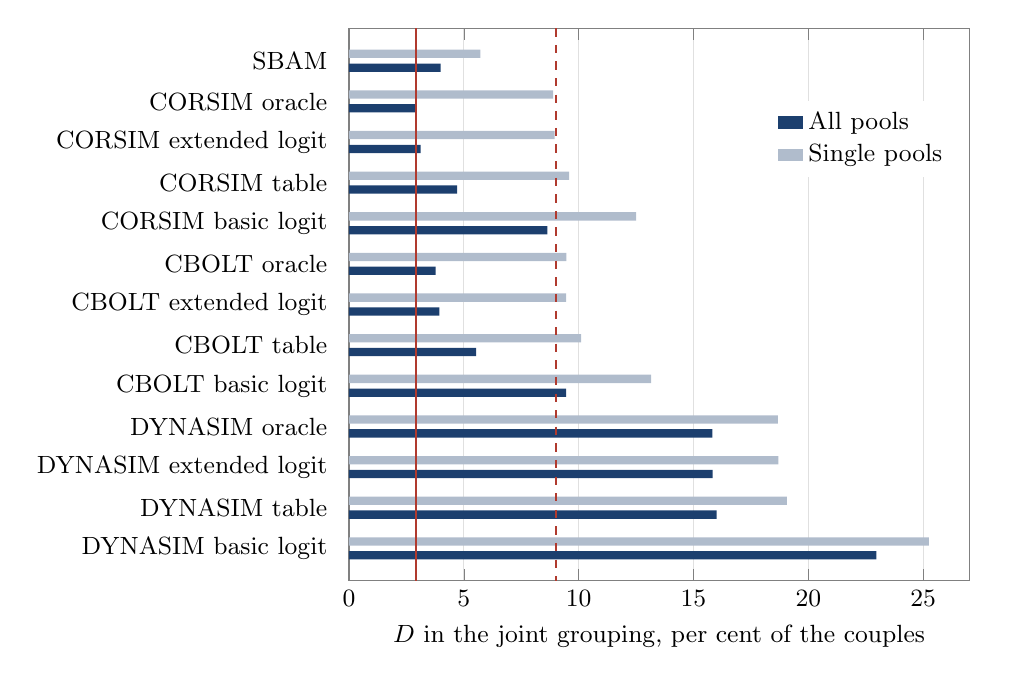
\begin{tikzpicture}
\begin{axis}[
  xbar, width=0.78\textwidth, height=8.6cm,
  bar width=3pt, xmin=0, xmax=27,
  xlabel={$D$ in the joint grouping, per cent of the couples},
  ytick={1,...,13}, y dir=reverse, ymin=0.2, ymax=13.8,
  yticklabels={SBAM,CORSIM oracle,CORSIM extended logit,CORSIM table,CORSIM basic logit,
    CBOLT oracle,CBOLT extended logit,CBOLT table,CBOLT basic logit,
    DYNASIM oracle,DYNASIM extended logit,DYNASIM table,DYNASIM basic logit},
  yticklabel style={font=\small}, xlabel style={font=\small}, xticklabel style={font=\small},
  xmajorgrids, grid style={black!12}, axis line style={black!50}, tick style={black!50},
  ytick style={draw=none},
  legend style={font=\small, draw=none, at={(0.98,0.80)}, anchor=east, legend cell align=left},
  legend image code/.code={\draw[#1, draw=none] (0cm,-0.08cm) rectangle (0.32cm,0.08cm);}]
\addplot[fill=accent, draw=none] coordinates {
  (3.99,1) (2.92,2) (3.12,3) (4.71,4) (8.64,5)
  (3.77,6) (3.94,7) (5.54,8) (9.45,9)
  (15.82,10) (15.83,11) (16.01,12) (22.96,13)};
\addplot[fill=accent!35, draw=none] coordinates {
  (5.72,1) (8.89,2) (8.95,3) (9.58,4) (12.50,5)
  (9.47,6) (9.45,7) (10.11,8) (13.15,9)
  (18.67,10) (18.69,11) (19.06,12) (25.25,13)};
\legend{All pools, Single pools}
\draw[second, thick] (axis cs:2.93,0.2) -- (axis cs:2.93,13.8);
\draw[second, thick, dashed] (axis cs:9.01,0.2) -- (axis cs:9.01,13.8);
\end{axis}
\end{tikzpicture}
\caption{Dissimilarity index in the joint grouping, baseline. The red lines show one draw from the
true model: 2.93 for all pools (solid) and 9.01 for single pools (dashed). The DYNASIM rule with
the distance function (50.5 and 51.4) is outside the figure.}
\label{fig:djoint}
\end{figure}

\textbf{SBAM hits the correct answer.} The partners have the same education in 55.6 per cent of
the couples and live in the same region in 77.0 per cent, against 55.4 and 76.7 in the correct
answer. The standard deviation of the age difference is 3.29 against 3.28. For all pools together
$D$ is 3.99 in the joint grouping, one percentage point above the floor of 2.93. The systematic
error is thus small but not zero. Section~\ref{sec:history} shows that it comes from the
sampling error in the historical table.

\textbf{In a single call SBAM deviates less than a random draw from the true model.} $D$ for
single pools is 5.72 for SBAM and 9.01 for one draw from the true model. The reason is the
systematic selection, which gives every cell its expected number of couples rounded up or down.
In the joint grouping this holds by construction. In the grouping by age, which is not aligned
with SBAM's sort order, $D$ for single pools is 3.57 for SBAM against 4.58 for one draw. A model
that uses SBAM therefore gets less random variation in its couples from year to year than the
real world has. For most uses of a projection model, less Monte Carlo noise is an advantage.

\textbf{The index matters more than the rule for CORSIM and CBOLT.} With the oracle index the
CORSIM rule is at the floor: $D$ is 2.92 for all pools. With the extended logit it is 3.12, with
the table index 4.71, and with the basic logit 8.64. The basic logit gives the same age pattern
to all ages, and on this market the spread of the age difference grows with age. The error of the
basic logit is in the age grouping ($D = 10.5$). Figure~\ref{fig:agegap} shows the result: too
few couples with a difference of 0--3 years and too many with a difference a few years outside
that range.

\textbf{With the same information, SBAM is more precise than the stochastic rules.} SBAM and the
table index use the same historical table. $D$ for all pools is 3.99 for SBAM, 4.71 for the
CORSIM rule and 5.54 for the CBOLT rule. For single pools the figures are 5.72, 9.58 and 10.11.
The table index is zero in the cells without historical couples, and the stochastic rules must
sometimes form a couple there anyway: 41 couples per pool with the CORSIM rule, 5 with the CBOLT
rule and 1,738 with the DYNASIM rule.

\textbf{The stochastic rules widen the age distribution slightly, also with a perfect index.}
With the oracle index the standard deviation of the age difference is 3.35 for the CORSIM rule
and 3.39 for the CBOLT rule, against 3.28 in the correct answer. The share of couples with an age
difference more than ten years from the typical two years is 0.61 and 0.63 per cent against
0.53. A likely reason is that the couples formed last are formed from the persons who are left.
The result agrees with the observation cited by Zinn (2012) that stochastic rules flatten the age
distribution, but the effect is small here.

\textbf{The CBOLT rule forms too few couples within regions.} With the oracle index, 74.9 per
cent of the couples are from the same region against 76.7, and $D$ in the region grouping is 1.82
for all pools against 0.21 for the CORSIM rule. Part of the error comes from every man meeting
the women in the same queue order. In a variant of the rule that lets each man start at a random
place in the queue, $D$ in the region grouping falls to 1.15 and the same-region share rises to
75.6 per cent. The variant is not part of the documented rule and was run only as a diagnostic.
The rest of the error is probably due to the rule being one-sided, since the CORSIM rule, which
treats the genders alike, does not have it. That explanation has not been tested.

\textbf{The DYNASIM rule sorts too weakly.} A man meets at most 10 or 20 women. Even with the
oracle index, only 66.9 per cent of the couples are from the same region, and $D$ is 15.8 for all
pools. With the distance function, which ignores the region, the regions are paired as at random.

\begin{figure}[H]
\centering
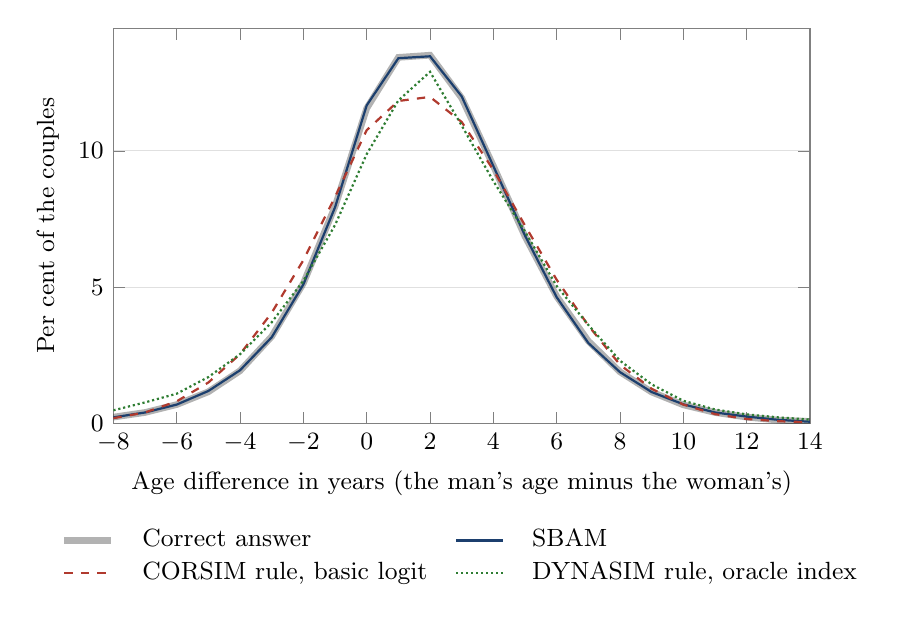
\begin{tikzpicture}
\begin{axis}[
  width=0.86\textwidth, height=6.6cm,
  xmin=-8, xmax=14, ymin=0, ymax=14.5,
  xlabel={Age difference in years (the man's age minus the woman's)}, ylabel={Per cent of the couples},
  xlabel style={font=\small}, ylabel style={font=\small}, ticklabel style={font=\small},
  ymajorgrids, grid style={black!12}, axis line style={black!50}, tick style={black!50},
  legend style={font=\small, draw=none, at={(0.5,-0.24)}, anchor=north, legend cell align=left,
    legend columns=2, column sep=8pt}]
\addplot[black, line width=2.4pt, opacity=0.3] coordinates {
  (-8,0.23) (-7,0.40) (-6,0.69) (-5,1.16) (-4,1.93) (-3,3.19) (-2,5.14) (-1,7.96) (0,11.56) (1,13.43) (2,13.51)
  (3,11.94) (4,9.45) (5,6.86) (6,4.66) (7,3.02) (8,1.89) (9,1.15) (10,0.68) (11,0.40) (12,0.23) (13,0.12) (14,0.07)};
\addplot[accent, thick] coordinates {
  (-8,0.22) (-7,0.40) (-6,0.69) (-5,1.19) (-4,1.95) (-3,3.16) (-2,5.10) (-1,7.93) (0,11.67) (1,13.40) (2,13.47)
  (3,12.00) (4,9.44) (5,6.89) (6,4.63) (7,2.95) (8,1.88) (9,1.15) (10,0.70) (11,0.40) (12,0.25) (13,0.13) (14,0.06)};
\addplot[second, thick, dashed] coordinates {
  (-8,0.19) (-7,0.40) (-6,0.81) (-5,1.50) (-4,2.54) (-3,4.06) (-2,5.99) (-1,8.31) (0,10.76) (1,11.83) (2,11.98)
  (3,11.06) (4,9.30) (5,7.26) (6,5.27) (7,3.59) (8,2.15) (9,1.27) (10,0.69) (11,0.34) (12,0.16) (13,0.08) (14,0.04)};
\addplot[third, thick, densely dotted] coordinates {
  (-8,0.48) (-7,0.77) (-6,1.09) (-5,1.70) (-4,2.54) (-3,3.71) (-2,5.23) (-1,7.28) (0,9.88) (1,11.85) (2,12.90)
  (3,10.93) (4,8.89) (5,7.04) (6,5.04) (7,3.61) (8,2.30) (9,1.43) (10,0.83) (11,0.51) (12,0.33) (13,0.22) (14,0.14)};
\legend{Correct answer, SBAM, CORSIM rule{,} basic logit, DYNASIM rule{,} oracle index}
\end{axis}
\end{tikzpicture}
\caption{Distribution of the age difference, baseline, all pools together. The curve for SBAM
lies on top of the correct answer.}
\label{fig:agegap}
\end{figure}

\subsection{A changed population}

Table~\ref{tab:change} shows the systematic error when the pool comes from a population that
differs from the one in the historical data.

\begin{table}[H]
\centering
\caption{$D$ in the joint grouping for all pools, by the degree of change in the population. The
last three lines show the share of couples with the same education, in per cent.}
\label{tab:change}
\small
\begin{tabular}{@{}l rrr@{}}
\toprule
 & Base population & Half change & Full change \\
\midrule
One draw from the true model & 2.93 & 2.95 & 2.96 \\
SBAM & 3.99 & 4.11 & 4.19 \\
CORSIM rule, extended logit & 3.12 & 3.14 & 3.19 \\
CORSIM rule, table index & 4.71 & 4.96 & 4.98 \\
CORSIM rule, basic logit & 8.64 & 8.68 & 8.63 \\
CBOLT rule, extended logit & 3.94 & 4.19 & 4.38 \\
CBOLT rule, table index & 5.54 & 5.61 & 5.92 \\
CBOLT rule, basic logit & 9.45 & 9.61 & 9.56 \\
DYNASIM rule, extended logit & 15.83 & 15.36 & 14.78 \\
\addlinespace
Same education: correct answer & 55.4 & 56.0 & 57.0 \\
Same education: SBAM & 55.6 & 56.1 & 57.1 \\
Same education: CORSIM rule, extended logit & 55.4 & 55.9 & 56.9 \\
\bottomrule
\end{tabular}
\end{table}

No method gets materially worse. SBAM follows the correct answer as the population changes: the
share of couples with the same education rises from 55.4 to 57.0 per cent in the correct answer
and from 55.6 to 57.1 per cent with SBAM, and $D$ rises from 3.99 to 4.19. This is what the
theory in Section~\ref{sec:methods} predicts. The CORSIM rule also follows, with $D$ unchanged
to within 0.3. The CBOLT rule loses a little, from 3.94 to 4.38 with the extended logit, and
the loss is in the region grouping.

The changed population therefore does not separate SBAM from a stochastic rule with a good index.
The stochastic rules have no theoretical guarantee here, but the proportional draws adapt to the
men and women who are available, and on this market that is enough.

\subsection{The amount of historical data}\label{sec:history}

Table~\ref{tab:history} and Figure~\ref{fig:history} show what happens when the historical data
shrink from 179,363 couples to 35,859 and to 3,624.

\begin{table}[H]
\centering
\caption{$D$ in the joint grouping by the amount of historical data: all pools, with single
pools in parentheses. One draw from the true model has 2.93 (9.01).}
\label{tab:history}
\small
\begin{tabular}{@{}l rrr@{}}
\toprule
 & 5 years & 1 year & 10 per cent of 1 year \\
Historical couples & 179,363 & 35,859 & 3,624 \\
\midrule
SBAM & 3.99 \ (5.72) & 8.75 \ (9.49) & 27.72 \ (28.05) \\
CORSIM rule, table index & 4.71 \ (9.58) & 9.12 \ (12.07) & 26.48 \ (27.50) \\
CBOLT rule, table index & 5.54 \ (10.11) & 9.68 \ (12.63) & 27.39 \ (28.30) \\
\addlinespace
CORSIM rule, basic logit & 8.64 \ (12.50) & 8.56 \ (12.46) & 8.63 \ (12.54) \\
CORSIM rule, extended logit & 3.12 \ (8.95) & 3.17 \ (8.95) & 4.10 \ (9.36) \\
CBOLT rule, extended logit & 3.94 \ (9.45) & 3.77 \ (9.37) & 4.44 \ (9.74) \\
\bottomrule
\end{tabular}
\end{table}

\begin{figure}[H]
\centering
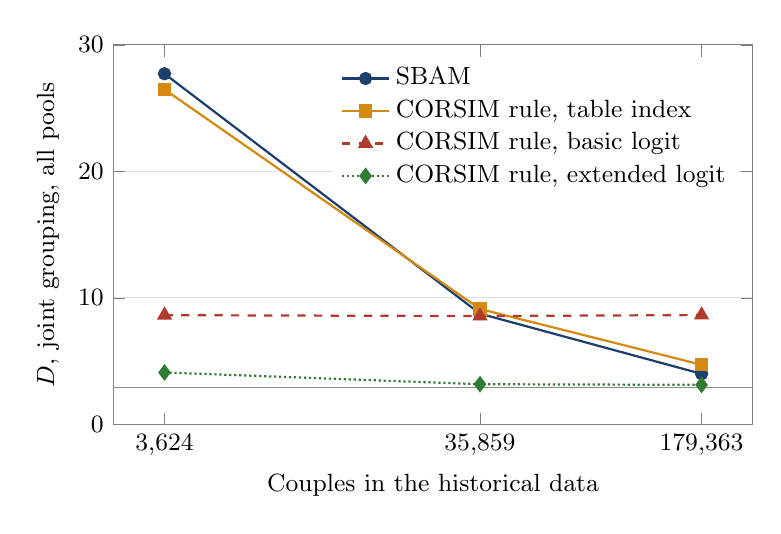
\begin{tikzpicture}
\begin{axis}[
  width=0.8\textwidth, height=6.4cm, xmode=log,
  xmin=2500, xmax=260000, ymin=0, ymax=30,
  xlabel={Couples in the historical data}, ylabel={$D$, joint grouping, all pools},
  xtick={3624,35859,179363}, xticklabels={{3,624},{35,859},{179,363}},
  xlabel style={font=\small}, ylabel style={font=\small}, ticklabel style={font=\small},
  ymajorgrids, grid style={black!12}, axis line style={black!50}, tick style={black!50},
  legend style={font=\small, draw=none, at={(0.98,0.97)}, anchor=north east, legend cell align=left}]
\addplot[accent, thick, mark=*, mark size=2pt] coordinates {(3624,27.72) (35859,8.75) (179363,3.99)};
\addplot[fourth, thick, mark=square*, mark size=2pt] coordinates {(3624,26.48) (35859,9.12) (179363,4.71)};
\addplot[second, thick, dashed, mark=triangle*, mark size=2.4pt, mark options={solid}] coordinates {(3624,8.63) (35859,8.56) (179363,8.64)};
\addplot[third, thick, densely dotted, mark=diamond*, mark size=2.4pt, mark options={solid}] coordinates {(3624,4.10) (35859,3.17) (179363,3.12)};
\addplot[black!45, thin] coordinates {(2500,2.93) (260000,2.93)};
\legend{SBAM, CORSIM rule{,} table index, CORSIM rule{,} basic logit, CORSIM rule{,} extended logit}
\end{axis}
\end{tikzpicture}
\caption{Systematic error and the amount of historical data. The grey line is one draw from the
true model (2.93).}
\label{fig:history}
\end{figure}

\textbf{SBAM needs a well-filled historical table.} With one year of data, $D$ for all pools
rises from 3.99 to 8.75. With a tenth of a year it is 27.7. The CORSIM rule with the table index
follows the same curve, so the error belongs to the table and not to the algorithm: the table has
176,400 cells, and with few couples most of what it shows is chance. This is also the source of
SBAM's systematic error with five years of data.

With the smallest data set SBAM has two further problems. On average 699 of the 71,836 persons in
a pool are of types that do not occur in the historical data, and they are left unmatched. And
the adjustment does not reach its tolerance in any of the ten pools. SBAM forms
98.5 per cent of the couples. With one year of data the adjustment reaches the tolerance in eight
pools of ten, and 99.99 per cent of the couples are formed.

\textbf{A logit index is insensitive to the amount of data.} The basic logit has nine parameters
and gives $D = 8.6$ with all three data sets. The extended logit gives 3.1, 3.2 and 4.1. With one
year of data the basic logit is as good as SBAM for all pools together (8.56 against 8.75),
though not in single pools (12.46 against 9.49). With a tenth of a year, any logit is far better
than the table.

The comparison of SBAM with the extended logit must be read with care. The extended logit was
specified with knowledge of the market. The result shows that smoothing can beat the raw table.
It does not show that a modeller would find the right specification in real data.

\subsection{Running time}

Table~\ref{tab:time} shows the running time in the baseline, and Figure~\ref{fig:time} shows how
it grows with the pool.

\begin{table}[H]
\centering
\caption{Running time of one call in the baseline pool of 71,836 persons: median over ten pools.
The stochastic rules are timed with the basic logit index. A look-up is one reading of the index
table.}
\label{tab:time}
\small
\begin{tabular}{@{}l rrr@{}}
\toprule
 & Milliseconds & Relative to SBAM & Look-ups per couple \\
\midrule
SBAM & 24.4 & 1 & -- \\
DYNASIM rule & 6.3 & 0.26 & 10 \\
CBOLT rule, by type & 16.5 & 0.68 & 443 \\
CORSIM rule, by type & 49.0 & 2.0 & 1,021 \\
CBOLT rule, by person & 820 & 34 & 17,983 \\
CORSIM rule, by person & 2,191 & 90 & 71,837 \\
\bottomrule
\end{tabular}
\end{table}

\textbf{SBAM takes 24 milliseconds for 72,000 persons.} Of these, 6 are spent in the adjustment,
which needs 53 passes on average, and 8 in forming the couples. The remaining 10 milliseconds
are the other steps of the call, such as sorting the persons into types. They were not timed
separately.

\textbf{By person, the CBOLT and CORSIM rules are 34 and 90 times slower than SBAM.} They take
0.8 and 2.2 seconds. The times are lower bounds for a model, because the index is read from a
table here. A model that computes the index for each pair from the characteristics of the two
persons does more work per pair.

\textbf{By type, the stochastic rules are as fast as SBAM.} The CBOLT rule takes 17 milliseconds
and the CORSIM rule 49. The by-type versions form the same couples as the by-person versions:
exactly the same for the CBOLT rule, in all ten pools, and the same in distribution for the
CORSIM rule ($D$ for all pools is 2.91 by person and 2.92 by type with the oracle index). The
index matters little for the time. With the other indices the CBOLT rule by type takes 18--19
milliseconds and the CORSIM rule by type 49--56.

\textbf{The DYNASIM rule is the fastest and the least precise.} It takes 6 milliseconds.

\begin{figure}[H]
\centering
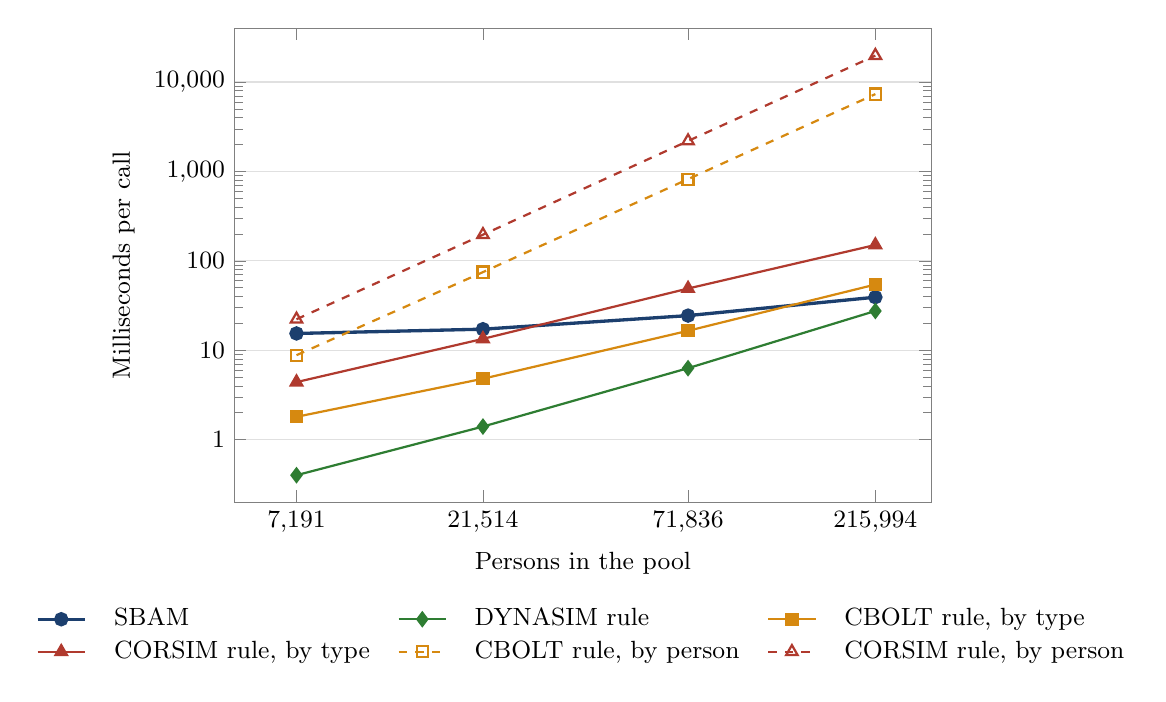
\begin{tikzpicture}
\begin{axis}[
  width=0.86\textwidth, height=7.6cm, xmode=log, ymode=log,
  xmin=5000, xmax=300000, ymin=0.2, ymax=40000,
  xlabel={Persons in the pool}, ylabel={Milliseconds per call},
  xtick={7191,21514,71836,215994}, xticklabels={{7,191},{21,514},{71,836},{215,994}},
  ytick={1,10,100,1000,10000}, yticklabels={1,10,100,{1,000},{10,000}},
  xlabel style={font=\small}, ylabel style={font=\small}, ticklabel style={font=\small},
  ymajorgrids, grid style={black!12}, axis line style={black!50}, tick style={black!50},
  legend style={font=\small, draw=none, at={(0.5,-0.2)}, anchor=north, legend cell align=left,
    legend columns=3, column sep=8pt}]
\addplot[accent, very thick, mark=*, mark size=2pt] coordinates {(7191,15.4) (21514,17.2) (71836,24.4) (215994,39.2)};
\addplot[third, thick, mark=diamond*, mark size=2.4pt] coordinates {(7191,0.4) (21514,1.4) (71836,6.3) (215994,27.5)};
\addplot[fourth, thick, mark=square*, mark size=2pt] coordinates {(7191,1.8) (21514,4.8) (71836,16.5) (215994,54.3)};
\addplot[second, thick, mark=triangle*, mark size=2.4pt] coordinates {(7191,4.4) (21514,13.4) (71836,49.0) (215994,150.5)};
\addplot[fourth, thick, dashed, mark=square, mark size=2pt, mark options={solid}] coordinates {(7191,8.8) (21514,74.8) (71836,820) (215994,7329)};
\addplot[second, thick, dashed, mark=triangle, mark size=2.4pt, mark options={solid}] coordinates {(7191,22.2) (21514,196) (71836,2191) (215994,19772)};
\legend{SBAM, DYNASIM rule, CBOLT rule{,} by type, CORSIM rule{,} by type, CBOLT rule{,} by person, CORSIM rule{,} by person}
\end{axis}
\end{tikzpicture}
\caption{Running time and the size of the pool. Both axes are logarithmic. The stochastic rules
are timed with the basic logit index. The by-person versions are timed in three pools in the
three settings that differ from the baseline.}
\label{fig:time}
\end{figure}

\textbf{SBAM's time grows least with the pool.} From 7,191 to 215,994 persons, a factor of 30,
SBAM goes from 15 to 39 milliseconds. Much of its work is done on the cells of the table, and
that work does not depend on the number of persons. The by-type rules grow in
proportion to the pool: the CBOLT rule from 1.8 to 54 milliseconds and the CORSIM rule from 4.4
to 151. The by-person rules grow with the square of the pool and reach 7.3 and 19.8 seconds.

In small pools SBAM is the slowest of the fast methods, because its work on the table costs
about the same however few persons there are. In a pool of 7,191 persons even the CBOLT rule by
person is faster (8.8 milliseconds). In the largest pool SBAM is faster than every stochastic
rule except the DYNASIM rule (28 milliseconds).

With less historical data SBAM gets faster, since there are fewer cells to adjust: 16
milliseconds with one year of data and 9 with a tenth of a year. The CBOLT rule with the table
index gets slower with the smallest data set, 53 milliseconds, because each man must pass more
women before one is accepted.

\section{Discussion}\label{sec:discussion}

\subsection{What the results show}

Three things decide the precision of a matching method: the information it uses, how it turns
the information into couples, and how much chance it adds.

On \emph{information}, SBAM and the table index use the raw historical table, and a logit index
uses a smoothed version of it. The raw table is right on average but noisy. The smoothed table is
stable but wrong where the model is wrong. With 179,363 historical couples in 176,400 cells, the
raw table beats a logit with nine parameters and loses narrowly to one with 31 well-chosen
parameters. With 3,624 couples the raw table is useless. Which side a real model is on depends on
the number of types and the amount of data. A production model can have many more types than the
420 used here, and its historical table is then more thinly filled.

On \emph{the algorithm}, SBAM fits both sides of the market at once and is exact on a market of
the Choo--Siow type. The CORSIM rule comes close: with a perfect index it reaches the floor, apart
from a slightly too wide age distribution. The CBOLT rule has a small systematic error, and the
DYNASIM rule a large one.

On \emph{chance}, SBAM adds less than any stochastic rule. In a single pool its deviation from
the correct answer is 64 per cent of that of the best stochastic rule in the joint grouping and
78 per cent in the grouping by age.

The speed of a method is decided by whether it works on persons or on types. SBAM has always
worked on types. The stochastic rules can do so too, at no cost in precision, and are then about
as fast as SBAM. Working on types requires that the compatibility index depends only on
characteristics that take few values. A model whose index uses continuous variables, such as
earnings, cannot group its persons in this way without rounding the variables.

\subsection{What the results do not show}

\begin{itemize}
\item \textbf{The market favours SBAM.} The artificial market is of the Choo--Siow type, where
biproportional adjustment is exactly right. If the preferences themselves change over time, the
historical table and a logit estimated on it are both wrong, and nothing here shows which is less
wrong.

\item \textbf{The stochastic rules are implemented from published descriptions,} not from the
code of the models. The models may differ from the descriptions in details that matter. The
scaling of the index in the DYNASIM rule is a choice made here.

\item \textbf{There is one set of historical data and ten pools per setting.} The floor moves
little between settings with the same pool size (2.93, 2.95 and 2.96), so chance in the pools is
small against the differences discussed. But a new draw of the historical data would move SBAM's
systematic error and that of the table index. No standard errors are computed.

\item \textbf{There are 420 types per gender.} With more types, the index table of the by-type
rules grows with the square of the number of types and their work in proportion to it. SBAM's
work grows with the number of non-zero cells. How the comparison turns out with many thousand
types has not been measured.

\item \textbf{The running times are from one machine,} whose speed varies. The ratios are more
reliable than the levels.

\item \textbf{The joint grouping is aligned with SBAM's sort order.} SBAM's advantage in single
pools is largest in that grouping.

\item \textbf{Some features of a real model are left out:} couples of the same gender, pools
with more men than women or the reverse, and a fallback for persons whose type is missing from
the historical data. SBAM needs such a fallback when the table is thin.
\end{itemize}

\section{Conclusion}

On a marriage market of the Choo--Siow type, with five years of historical data, the new
implementation of SBAM reproduces the correct couple table more precisely than any stochastic
rule that uses the same historical table, and with less random variation from call to call. A
call takes 24 milliseconds for a pool of 72,000 persons and 39 milliseconds for a pool three
times as large.

Stochastic matching as described in the literature, person by person, is 34 to 90 times slower
at the baseline pool size and 190 to 500 times slower in the largest pool. Implemented on
types, the CBOLT and CORSIM rules form the same couples at about the speed of SBAM. Their
precision then depends on the index. With a parsimonious logit the error is more than twice that
of SBAM. With a well-specified logit the CORSIM rule has a slightly smaller systematic error
than SBAM. The DYNASIM rule is fast but sorts the couples too weakly with any index.

SBAM's weak point is thin historical data. With 3,624 historical couples its error is more than
three times that of a logit index, and it cannot place the persons whose type is missing from
the table. A
model with many types and few observed couples should either smooth the historical table before
SBAM uses it or use a parametric index.

\appendix

\section{The artificial market}\label{app:market}

A type is a combination of age $a \in \{20,\dots,54\}$, education $e \in \{1,2,3\}$ and region
$r \in \{1,2,3,4\}$. For a man of type $x$ and a woman of type $y$, with age difference
$g = a_x - a_y$ and mean age $\bar{a} = (a_x + a_y)/2$,
\begin{equation*}
\log K_{xy} = \kappa - 0.035\,(a_x - 20) - 0.045\,(a_y - 20) - \frac{(g-2)^2}{2\,\tau^2}
  + \rho^E_{e_x e_y} + \rho^R_{r_x r_y}, \qquad \tau = 2 + 0.12\,(\bar{a} - 20).
\end{equation*}
The education term $\rho^E$ is 0.8, 0.5 and 0.9 when both have the lowest, the middle and the
highest education, $-0.9$ when one has the lowest and the other the highest, and 0 otherwise. The
region term $\rho^R$ is 0 within a region, $-1.5$ between regions 1 and 2, and $-2.6$ between
other regions. The constant $\kappa = -4.5616$ is set so that 12 per cent of the single men form
a couple in a year.

The number of singles of a type is proportional to $w^A \cdot w^R \cdot w^E$, with $d = a - 20$,
$f = 1$ for women and 0 for men, $h = 1$ in region 1 and 0 elsewhere, $\Lambda(z) = 1/(1+e^{-z})$
and the degree of change $c$ (0 in the base population, 1 with the full change):
\begin{align*}
w^A &= e^{-(0.06 - 0.035c)\,d} + 0.25 + 0.25c, \\
w^R &= (0.35 + 0.10c,\; 0.25,\; 0.25 - 0.05c,\; 0.15 - 0.05c) \text{ for regions 1--4}, \\
P(\text{highest}) &= \Lambda\bigl(-1.2 + 0.6f - 0.02d + 0.5h + c\,(0.4 + 0.4f)\bigr), \\
P(\text{lowest}) &= \bigl(1 - P(\text{highest})\bigr)\,\Lambda\bigl(-1.0 - 0.3f + 0.02d - 0.3h - 0.4c\bigr).
\end{align*}
There are 300,000 singles of each gender before rounding. With the full change the market forms
33,074 couples a year, with the half change 34,602.

\section{The logit models}\label{app:logit}

Table~\ref{tab:logit} shows the estimates on the five years of historical data: 179,363 couples
among $179{,}363^2 = 32.2$ billion potential pairs. The log-likelihood is $-2{,}108{,}524$ for
the basic specification and $-2{,}072{,}195$ for the extended one. The extended specification
has 13 further parameters, one for each combination of the man's and the woman's region that is
not identified by the two region parameters in the table. They are between $-0.84$ and $0.01$.

\begin{table}[H]
\centering
\caption{Logit models on potential pairs, five years of historical data. Mean age is the mean
age of the two partners minus 37, divided by 10. Education levels are numbered 1--3.}
\label{tab:logit}
\small
\begin{tabular}{@{}l rr@{}}
\toprule
 & Basic & Extended \\
\midrule
Constant & $-12.106$ & $-11.861$ \\
Age difference (man minus woman) & $0.142$ & $0.137$ \\
Age difference squared & $-0.038$ & $-0.029$ \\
Woman two education levels higher & $-1.362$ & $-1.171$ \\
Woman one education level higher & $-0.608$ & $-0.459$ \\
Woman one education level lower & $-0.720$ & $-0.593$ \\
Woman two education levels lower & $-1.543$ & $-1.363$ \\
Same region & $2.450$ & $2.779$ \\
Neighbouring regions (1 and 2) & $0.782$ & $0.527$ \\
Mean age & & $0.654$ \\
Mean age squared & & $0.367$ \\
Age difference $\times$ mean age & & $-0.082$ \\
Age difference squared $\times$ mean age & & $0.022$ \\
Age difference squared $\times$ mean age squared & & $-0.011$ \\
Both have education 1 & & $0.548$ \\
Both have education 3 & & $0.343$ \\
Man education 1, woman education 2 & & $0.131$ \\
Man education 2, woman education 1 & & $0.158$ \\
Region of the man and the woman, 13 combinations & & (see text) \\
\bottomrule
\end{tabular}
\end{table}

\section*{References}

\begin{list}{}{\setlength{\leftmargin}{1.5em}\setlength{\itemindent}{-1.5em}\setlength{\itemsep}{3pt}\setlength{\parsep}{0pt}\small}

\item Bouffard, N., R. Easther, T. Johnson, R. J. Morrison and J. Vink (2001). Matchmaker,
matchmaker, make me a match. \emph{Brazilian Electronic Journal of Economics}, 4(2).

\item Choo, E. and A. Siow (2006). Who marries whom and why. \emph{Journal of Political Economy},
114(1), 175--201.

\item Decker, C., E. H. Lieb, R. J. McCann and B. K. Stephens (2013). Unique equilibria and
substitution effects in a stochastic model of the marriage market. \emph{Journal of Economic
Theory}, 148(2), 778--792.

\item Deming, W. E. and F. F. Stephan (1940). On a least squares adjustment of a sampled
frequency table when the expected marginal totals are known. \emph{Annals of Mathematical
Statistics}, 11, 427--444.

\item Duncan, O. D. and B. Duncan (1955). A methodological analysis of segregation indexes.
\emph{American Sociological Review}, 20(2), 210--217.

\item Easther, R. and J. Vink (2000). A stochastic marriage market for CORSIM. Technical paper,
Strategic Forecasting.

\item Gale, D. and L. S. Shapley (1962). College admissions and the stability of marriage.
\emph{American Mathematical Monthly}, 69(1), 9--15.

\item Galichon, A. and B. Salanié (2022). Cupid's invisible hand: Social surplus and
identification in matching models. \emph{Review of Economic Studies}, 89(5), 2600--2629.

\item Kalmijn, M. (1998). Intermarriage and homogamy: Causes, patterns, trends. \emph{Annual
Review of Sociology}, 24, 395--421.

\item Leblanc, N., R. Morrison and H. Redway (2009). A match made in silicon: Marriage matching
algorithms for dynamic microsimulation. Paper presented at the 2nd General Conference of the
International Microsimulation Association, Ottawa, 8--10 June.

\item Li, J. and C. O'Donoghue (2013). A survey of dynamic microsimulation models: uses, model
structure and methodology. \emph{International Journal of Microsimulation}, 6(2), 3--55.

\item Madow, W. G. and L. H. Madow (1944). On the theory of systematic sampling, I. \emph{Annals
of Mathematical Statistics}, 15, 1--24.

\item Mare, R. D. (1991). Five decades of educational assortative mating. \emph{American
Sociological Review}, 56(1), 15--32.

\item de Menten, G., G. Dekkers, G. Bryon, P. Liégeois and C. O'Donoghue (2014). LIAM2: a new
open source development tool for discrete-time dynamic microsimulation models. \emph{Journal of
Artificial Societies and Social Simulation}, 17(3), 9.

\item Orcutt, G. H., S. Caldwell and R. Wertheimer II (1976). \emph{Policy Exploration Through
Microanalytic Simulation}. Washington, DC: Urban Institute Press.

\item Perese, K. (2002). Mate matching for microsimulation models. Technical Paper 2002-3,
Long-Term Modeling Group, Congressional Budget Office, Washington, DC.

\item Stephensen, P. and T. Markeprand (2013). SBAM: An algorithm for pair matching. DREAM
Working Paper 2013:3.

\item Zinn, S. (2012). A mate-matching algorithm for continuous-time microsimulation models.
\emph{International Journal of Microsimulation}, 5(1), 31--51.

\end{list}

\end{document}
